\documentclass[notes,11pt, aspectratio=169]{beamer}

\usepackage{pgfpages}
% These slides also contain speaker notes. You can print just the slides,
% just the notes, or both, depending on the setting below. Comment out the want
% you want.
\setbeameroption{hide notes} % Only slide
%\setbeameroption{show only notes} % Only notes
%\setbeameroption{show notes on second screen=right} % Both

\usepackage{helvet}
\usepackage[default]{lato}
\usepackage{array}
\usepackage{tgbonum}

\usepackage{tikz}
\usepackage{verbatim}
\setbeamertemplate{note page}{\pagecolor{yellow!5}\insertnote}
\usetikzlibrary{positioning}
\usetikzlibrary{snakes}
\usetikzlibrary{calc}
\usetikzlibrary{arrows}
\usetikzlibrary{decorations.markings}
\usetikzlibrary{shapes.misc}
\usetikzlibrary{matrix,shapes,arrows,fit,tikzmark}
\usepackage{amsmath}
\usepackage{mathpazo}
\usepackage{hyperref}
\usepackage{lipsum}
\usepackage{multimedia}
\usepackage{graphicx}
\usepackage{multirow}
\usepackage{graphicx}
\usepackage{dcolumn}
\usepackage{bbm}
\newcolumntype{d}[0]{D{.}{.}{5}}

\usepackage{changepage}
\usepackage{appendixnumberbeamer}
\newcommand{\beginbackup}{
   \newcounter{framenumbervorappendix}
   \setcounter{framenumbervorappendix}{\value{framenumber}}
   \setbeamertemplate{footline}
   {
     \leavevmode%
     \hline
     box{%
       \begin{beamercolorbox}[wd=\paperwidth,ht=2.25ex,dp=1ex,right]{footlinecolor}%
%         \insertframenumber  \hspace*{2ex} 
       \end{beamercolorbox}}%
     \vskip0pt%
   }
 }
\newcommand{\backupend}{
   \addtocounter{framenumbervorappendix}{-\value{framenumber}}
   \addtocounter{framenumber}{\value{framenumbervorappendix}} 
}


\usepackage{graphicx}
\usepackage[space]{grffile}
\usepackage{booktabs}
\newcommand\independent{\protect\mathpalette{\protect\independenT}{\perp}}
\def\independenT#1#2{\mathrel{\rlap{$#1#2$}\mkern2mu{#1#2}}}
\DeclareMathOperator{\Supp}{Supp}


\newtheorem{assN}{Assumption}
% These are my colors -- there are many like them, but these ones are mine.
\definecolor{blue}{RGB}{0,114,178}
\definecolor{red}{RGB}{213,94,0}
\definecolor{yellow}{RGB}{240,228,66}
\definecolor{green}{RGB}{0,158,115}

\hypersetup{
  colorlinks=false,
  linkbordercolor = {white},
  linkcolor = {blue}
}


%% I use a beige off white for my background
\definecolor{MyBackground}{RGB}{255,253,218}

%% Uncomment this if you want to change the background color to something else
%\setbeamercolor{background canvas}{bg=MyBackground}

%% Change the bg color to adjust your transition slide background color!
\newenvironment{transitionframe}{
  \setbeamercolor{background canvas}{bg=yellow}
  \begin{frame}}{
    \end{frame}
}

\setbeamercolor{frametitle}{fg=blue}
\setbeamercolor{title}{fg=black}
\setbeamertemplate{footline}[frame number]
\setbeamertemplate{navigation symbols}{} 
\setbeamertemplate{itemize items}{-}
\setbeamercolor{itemize item}{fg=blue}
\setbeamercolor{itemize subitem}{fg=blue}
\setbeamercolor{enumerate item}{fg=blue}
\setbeamercolor{enumerate subitem}{fg=blue}
\setbeamercolor{button}{bg=MyBackground,fg=blue,}



% If you like road maps, rather than having clutter at the top, have a roadmap show up at the end of each section 
% (and after your introduction)
% Uncomment this is if you want the roadmap!
% \AtBeginSection[]
% {
%    \begin{frame}
%        \frametitle{Roadmap of Talk}
%        \tableofcontents[currentsection]
%    \end{frame}
% }
\setbeamercolor{section in toc}{fg=blue}
\setbeamercolor{subsection in toc}{fg=red}
\setbeamersize{text margin left=1em,text margin right=1em} 

\newenvironment{wideitemize}{\itemize\addtolength{\itemsep}{10pt}}{\enditemize}

\usepackage{environ}
\NewEnviron{videoframe}[1]{
  \begin{frame}
    \vspace{-8pt}
    \begin{columns}[onlytextwidth, T] % align columns
      \begin{column}{.70\textwidth}
        \begin{minipage}[t][\textheight][t]
          {\dimexpr\textwidth}
          \vspace{8pt}
          \hspace{4pt} {\Large \sc \textcolor{blue}{#1}}
          \vspace{8pt}
          
          \BODY
        \end{minipage}
      \end{column}%
      \hfill%
      \begin{column}{.38\textwidth}
        \colorbox{green!20}{\begin{minipage}[t][1.2\textheight][t]
            {\dimexpr\textwidth}
            Face goes here
          \end{minipage}}
      \end{column}%
    \end{columns}
  \end{frame}
}

\title[]{\textcolor{blue}{Canonical Research Designs VI:\\ Examiner Designs (aka Judge IV, aka leniency IV) }}
\author[PGP]{}
\institute[FRBNY]{\small{\begin{tabular}{c}
  Paul Goldsmith-Pinkham  \\
\end{tabular}}}

\date{\today}

\begin{document}

%%% TIKZ STUFF
\tikzset{   
        every picture/.style={remember picture,baseline},
        every node/.style={anchor=base,align=center,outer sep=1.5pt},
        every path/.style={thick},
        }
\newcommand\marktopleft[1]{%
    \tikz[overlay,remember picture] 
        \node (marker-#1-a) at (-.3em,.3em) {};%
}
\newcommand\markbottomright[2]{%
    \tikz[overlay,remember picture] 
        \node (marker-#1-b) at (0em,0em) {};%
}
\tikzstyle{every picture}+=[remember picture] 
\tikzstyle{mybox} =[draw=black, very thick, rectangle, inner sep=10pt, inner ysep=20pt]
\tikzstyle{fancytitle} =[draw=black,fill=red, text=white]
%%%% END TIKZ STUFF

% Title Slide
\begin{frame}
\maketitle
\end{frame}

\begin{frame}{Roadmap for Today}
  \begin{wideitemize}
  \item Today we're focusing on a particular research design: the examiner design
  \item Like many of the designs we are studying, they have shown up
    in papers for a while, but have really started to take off
    recently with the rise of high-quality administrative microdata.
  \item Key issues we'll touch on:
    \begin{itemize}
    \item Identification: what are we getting at?
    \item Estimation: What's the best estimation method for using the
      examiner design?
    \item Inference: How should we do inference?
    \end{itemize}
  \end{wideitemize}
\end{frame}

\begin{frame}{High-level description of examiner design}
    \begin{columns}[onlytextwidth, T] % align columns
      \begin{column}{.6\textwidth}
        \begin{wideitemize}
        \item In many applications, there is an administrator, judge,
          or monitor who plays an important role in deciding an
          outcome
        \item These outcomes include:
          \begin{itemize}
          \item bail
          \item banktrupcy
          \item getting a loan
          \item parole
          \item disability insurance
          \item patent granting
          \item cancer screening
          \end{itemize}
        \item In many cases, this examiner is effectively randomly
          assigned, \emph{and} there is wide-range of differences (and
          discretion) in how likely they are to decide the outcome
        \end{wideitemize}
      \end{column}%
      \hfill%
      \begin{column}{.4\textwidth}
        \only<2->{
        \begin{wideitemize}
        \item Key ingredients:
          \begin{enumerate}
          \item random assignment of examiner
          \item discretion over a (typically binary) outcome
          \item heterogeneity in behavior
          \end{enumerate}
        \end{wideitemize}
        }
      \end{column}%
    \end{columns}
\end{frame}

\begin{frame}{Consider two examples}
  \begin{columns}[onlytextwidth, T] % align columns
    \begin{column}{.50\textwidth}
      \begin{wideitemize}
      \item Example 1: Bail setting in Philadelphia (Stevenson (2018))
      \item After you're arrested, you can be:
        \begin{itemize}
        \item held in jail
        \item released on bail (you pay \$)
        \item released on recognizance (no bail \$)
        \end{itemize}
      \item This decision is made by one of six magistrates at
        preliminary hearings
        \begin{itemize}
        \item The particular magistrate that a defendant faces
          depends on a rotating schedule
        \item Hence, the randomness occurs from \emph{the time of
            day}
        \end{itemize}
      \end{wideitemize}
    \end{column}%
    \hfill%
    \begin{column}{.5\textwidth}
      \only<1>{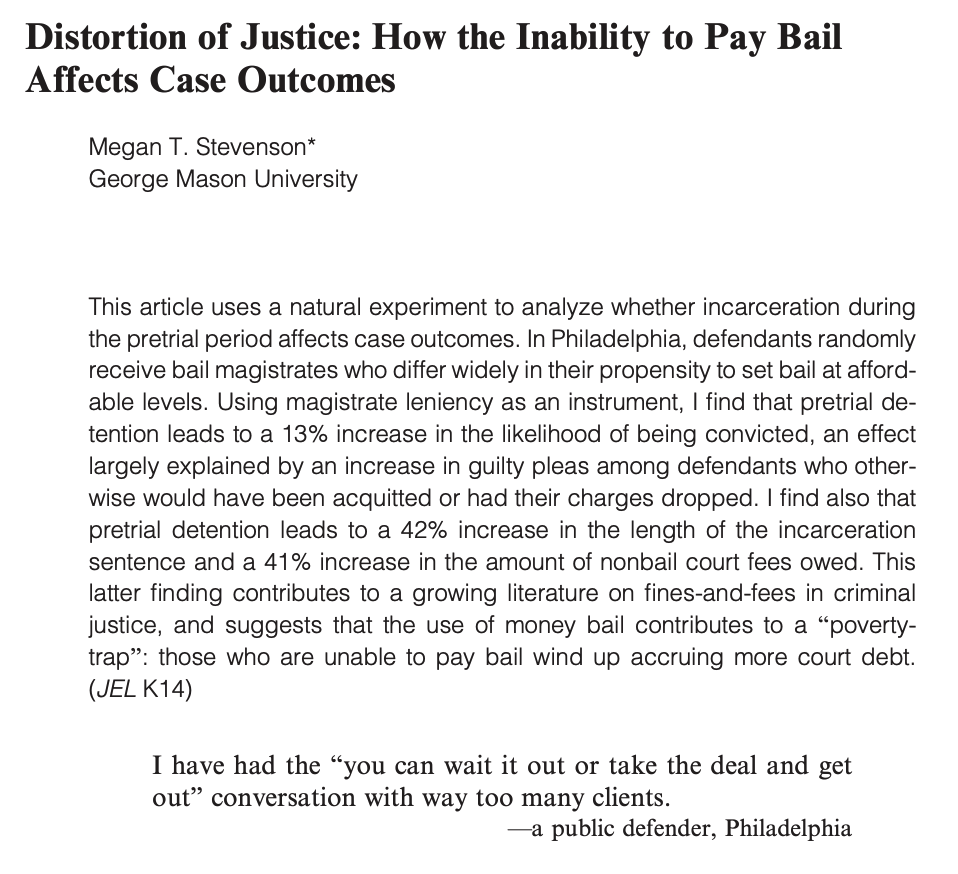
\includegraphics[width=\linewidth]{images/stevenson_1.png}}
      \only<2>{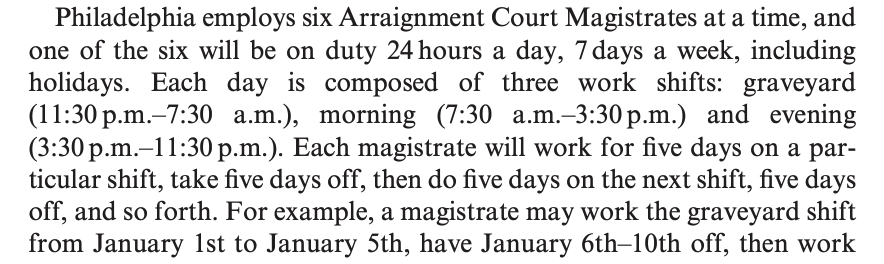
\includegraphics[width=\linewidth]{images/stevenson_2a.png}\\
        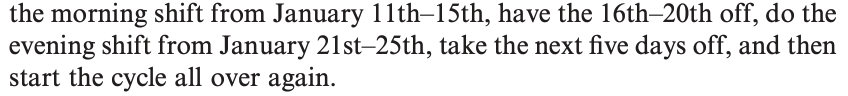
\includegraphics[width=\linewidth]{images/stevenson_2b.png}}
    \end{column}%
  \end{columns}
\end{frame}

\begin{frame}{Consider two examples}
  \begin{columns}[onlytextwidth, T] % align columns
    \begin{column}{.50\textwidth}
      \begin{wideitemize}
      \item Example 2: Bankruptcy judges in Chapter 13 (Dobbie et al.(2017))
      \item When you file for Chapter 13 bankruptcy, you file a
        repayment plan to be approved by a judge
      \item This decision is made by different judges staffed at a
        court on a given day
        \begin{itemize}
        \item The assigned judge is done randomly by the court
        \item Hence, the randomness occurs within \emph{location-time}
          of filing
        \end{itemize}
      \end{wideitemize}
    \end{column}%
    \hfill%
    \begin{column}{.5\textwidth}
      \only<1>{
\includegraphics[width=\linewidth]{images/dgy_1.png}}
      \only<2>{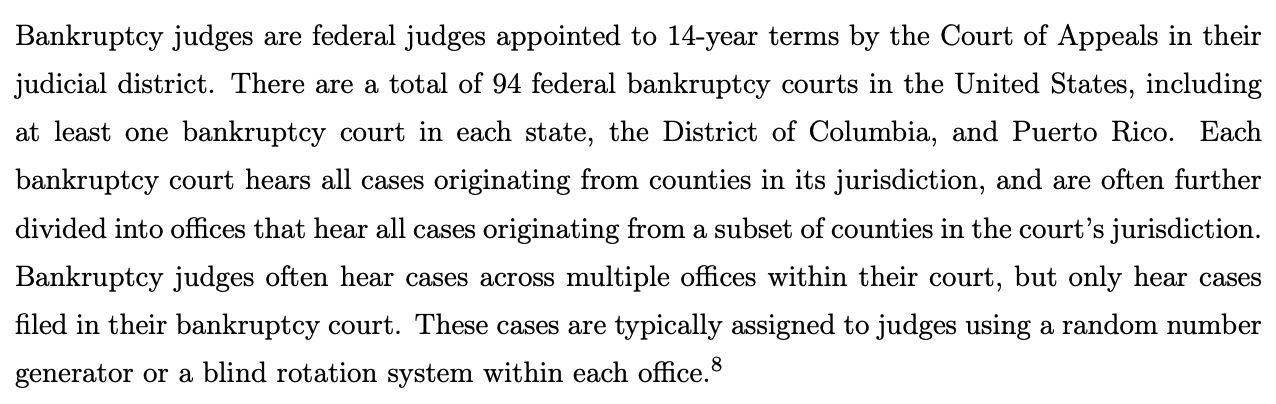
\includegraphics[width=\linewidth]{images/dgy_2.png}}      
    \end{column}%
  \end{columns}
\end{frame}

\begin{frame}{Notation}
  \begin{wideitemize}
  \item Before we get to intuition, let's start with some notation
  \item We consider $n$ individuals indexed by $i$, with two outcomes: $D_{i}$  and $Y_{i}$
  \item Each individual is assigned to one of $K$ examiners: $Q_{i} \in \{0, \ldots, K-1\}$
  \item Hence, very easy to consider the potential outcomes $D_{i}(q)$
    for each of the potential exmainers, where we observe only one!
    \begin{itemize}
    \item If $K=2$, this is just our simple binary case.
    \item With  $K > 2$, it becomes more complicated
    \item Note that there's no meaningful ordering to the $K$ exmainers 
    \end{itemize}
  \item We can \emph{also} consider the potential outcomes $Y_{i}(q)$. What are we ignoring?
    \pause
    \begin{itemize}
    \item Potential impact of $D_{i}$ on $Y_{i}$. When we do IV, we'll
      need to consider $Y_{i}(D_{i}(Q_{i}), Q_{i})$, and then shut
      down the direct effect of $Q_{i}$ in order to do IV
    \end{itemize}
  \end{wideitemize}
\end{frame}

\begin{frame}{Intuition}
  \begin{wideitemize}
  \item First consider the variation in $D_{i}$ across the $Q_{i}$.
    \begin{itemize}
    \item Conditional on some covariates $W_{i}$, we assume that
      strong ignorability holds
    \end{itemize}
  \item If $W_{i}$ is just a constant, then we can consider
    $\tau_{q, q'} = E(D_{i} | Q_{i} = q) - E(D_{i} | Q_{i} = q')$
    \begin{itemize}
    \item This is the relative effect of judge $q$ vs. $q'$ on bail
      decisions or bankruptcy discharge 
    \end{itemize}
  \item We have an RCT, but with judges!
  \item Useful to also define $\mu_{D}(q) = E(D_{i}| Q_{i} = q)$
    \begin{itemize}
    \item     $\hat{\mu}_{D}(q)$ is the corresponding empirical estimate
    \end{itemize}
  \end{wideitemize}
\end{frame}

\begin{frame}{What is this measure? }
  \begin{wideitemize}
  \item In the context of bankruptcy or bail judges, $\mu_{D}(q)$
    measures judge $q$'s \emph{leniency} -- e.g. their average
    propensity
  \item We can literally estimate this with a simple linear regression of dummies! E.g. let $\mathcal{Q}_{i}$ be the set of dummies for $Q_{i}$:
    \begin{equation*}
      D_{i} = \mathcal{Q}_{i}\mu_{D} + u_{i}
    \end{equation*}
  \item Note that given the simplicity of this measure, the $\mu_{D}$ are equivalent to the predicted values for $D_{i}$
    \begin{itemize}
    \item E.g. $\hat{D}$ from the regression on $\mathcal{Q}_{i}$
    \end{itemize}
  \item This predicted measure dovetails exactly into the measure that
    papers have historically used!
  \end{wideitemize}
\end{frame}

\begin{frame}{What's the instrument that people have used?}
    \begin{columns}[onlytextwidth, T] % align columns
      \begin{column}{.5\textwidth}
        \begin{wideitemize}
        \item In many papers, the measure that has been used is a
          ``leniency'' metric for judges: e.g. the $\hat{D}_{i}$
        \item This is the overall average leniency across judges in
          DGPY [note, not observation weighted -- hence outliers]
        \item What's the problem with just the overall, in the DGPY
          context?
          \begin{itemize}
          \item Judges are not random overall -- location (and time)
            specific
          \end{itemize}
        \item Importantly, the average judge characteristic may
          capture location specific features
          \begin{itemize}
          \item Control for $W_{i}$
          \end{itemize}
        \end{wideitemize}
      \end{column}%
      \hfill%
      \begin{column}{.5\textwidth}
        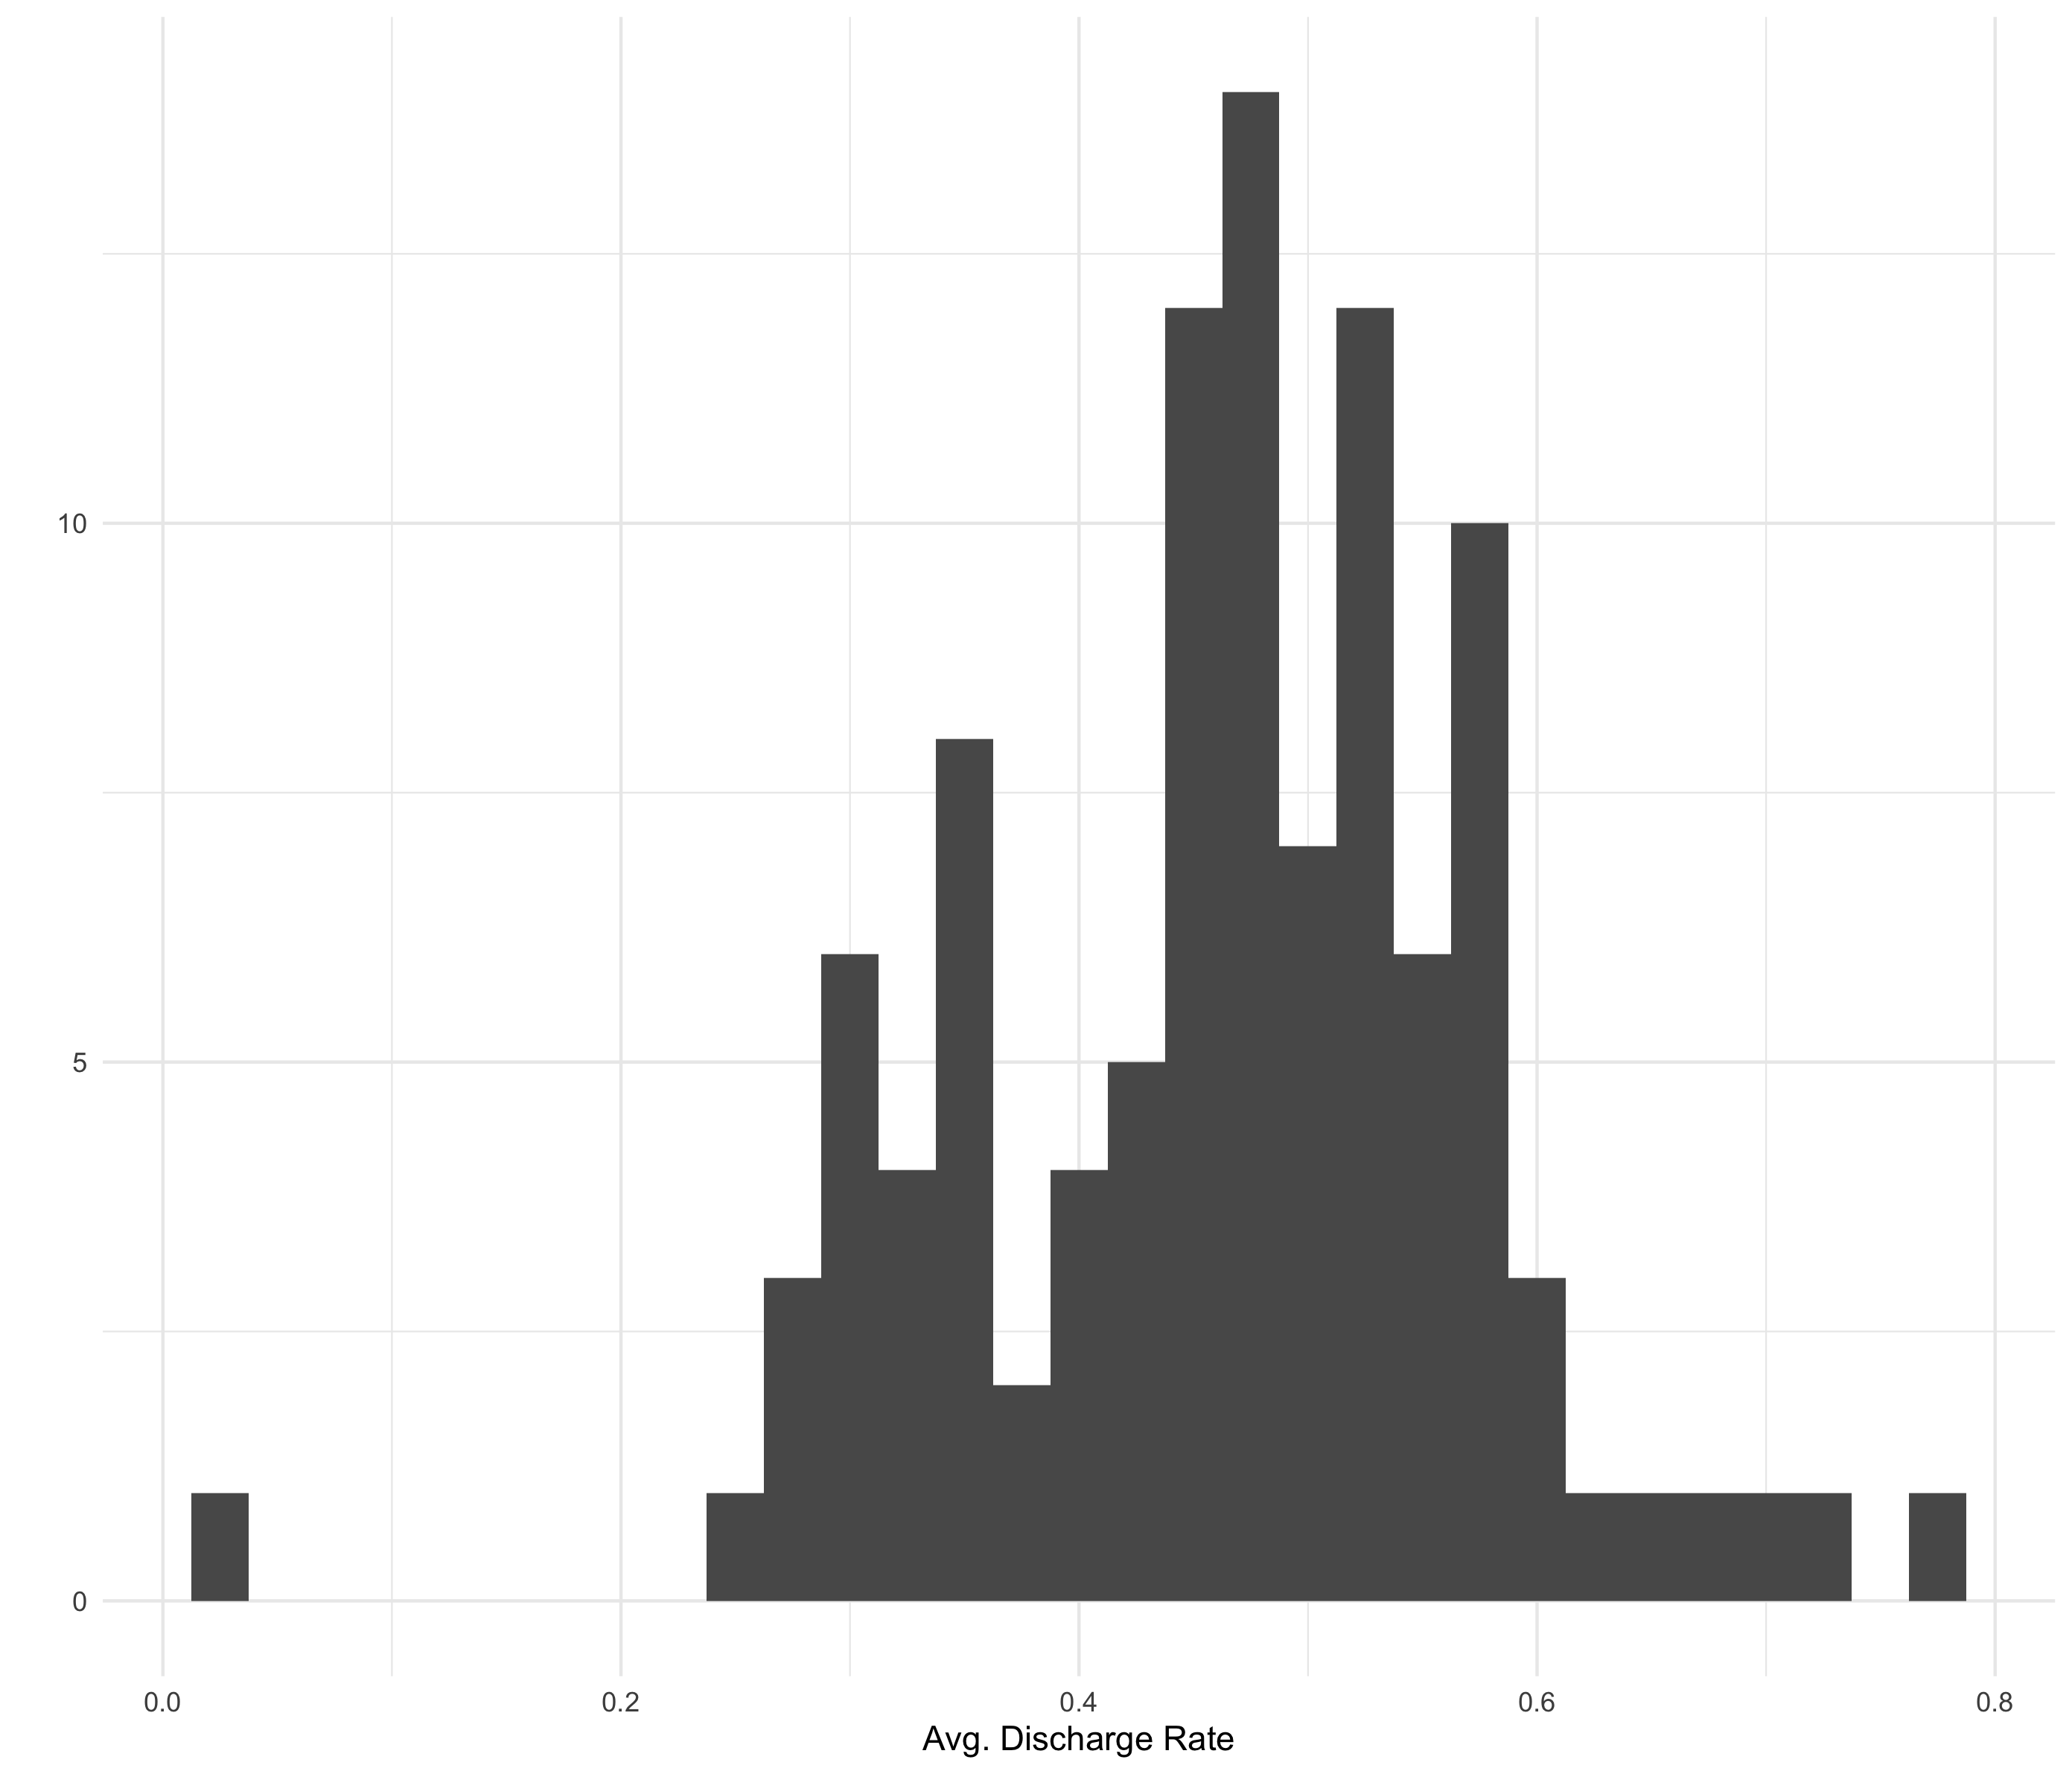
\includegraphics[width=\linewidth]{images/leniency_overall.png}
      \end{column}%
    \end{columns}
\end{frame}

\begin{frame}{How to incorporate $W_{i}$?}
  \begin{wideitemize}
  \item Now consider the simple linear regression with $W_{i}$:
    \begin{equation*}
      D_{i} = \mathcal{Q}_{i}\mu_{D} + W_{i}\gamma +  u_{i}
    \end{equation*}
  \item Now, the $\mu_{D}$ are equivalent to the predicted values for
    $D_{i}$ \emph{after residualizing out for $W_{i}$} (which usually
    includes a constant)
    \begin{itemize}
    \item E.g. $\hat{D}^{\perp}$ from the regression on $\mathcal{Q}_{i}^{\perp}$
    \item Call this measure $Z_{i} = \hat{D}^{\perp}$ our leniency measure
    \end{itemize}
  \item This captures the average variation in leniency within the average of a location
    \begin{itemize}
    \item In the simple case where judges are nested within courts,
      this just captures variation across $Q$ due to judge specific
      random variation
    \item Mechanically, this would literally capture
      \begin{align*}
        \hat{D}^{\perp} &= n^{-1}\left(\underbrace{\sum_{i}1(Q_{i} = q)D_{i}}_{\text{judge mean}} - \underbrace{\sum_{i}1(W_{i} = w)D_{i}}_{\text{location mean}}\right)
      \end{align*}
    \end{itemize}
  \end{wideitemize}
\end{frame}


\begin{frame}{What's the instrument that people have used?}
    \begin{columns}[onlytextwidth, T] % align columns
      \begin{column}{.5\textwidth}
        \begin{wideitemize}
        \item Once you do this exercise with judge leniency, you get a
          much more recentered object
        \item This captures across location differences, and give true variation
        \item Point worth noting -- due to the location effect, we
          can't estimate the ``true'' judge leniency -- just relative
          leniency within an office
        \end{wideitemize}
      \end{column}%
      \hfill%
      \begin{column}{.5\textwidth}
        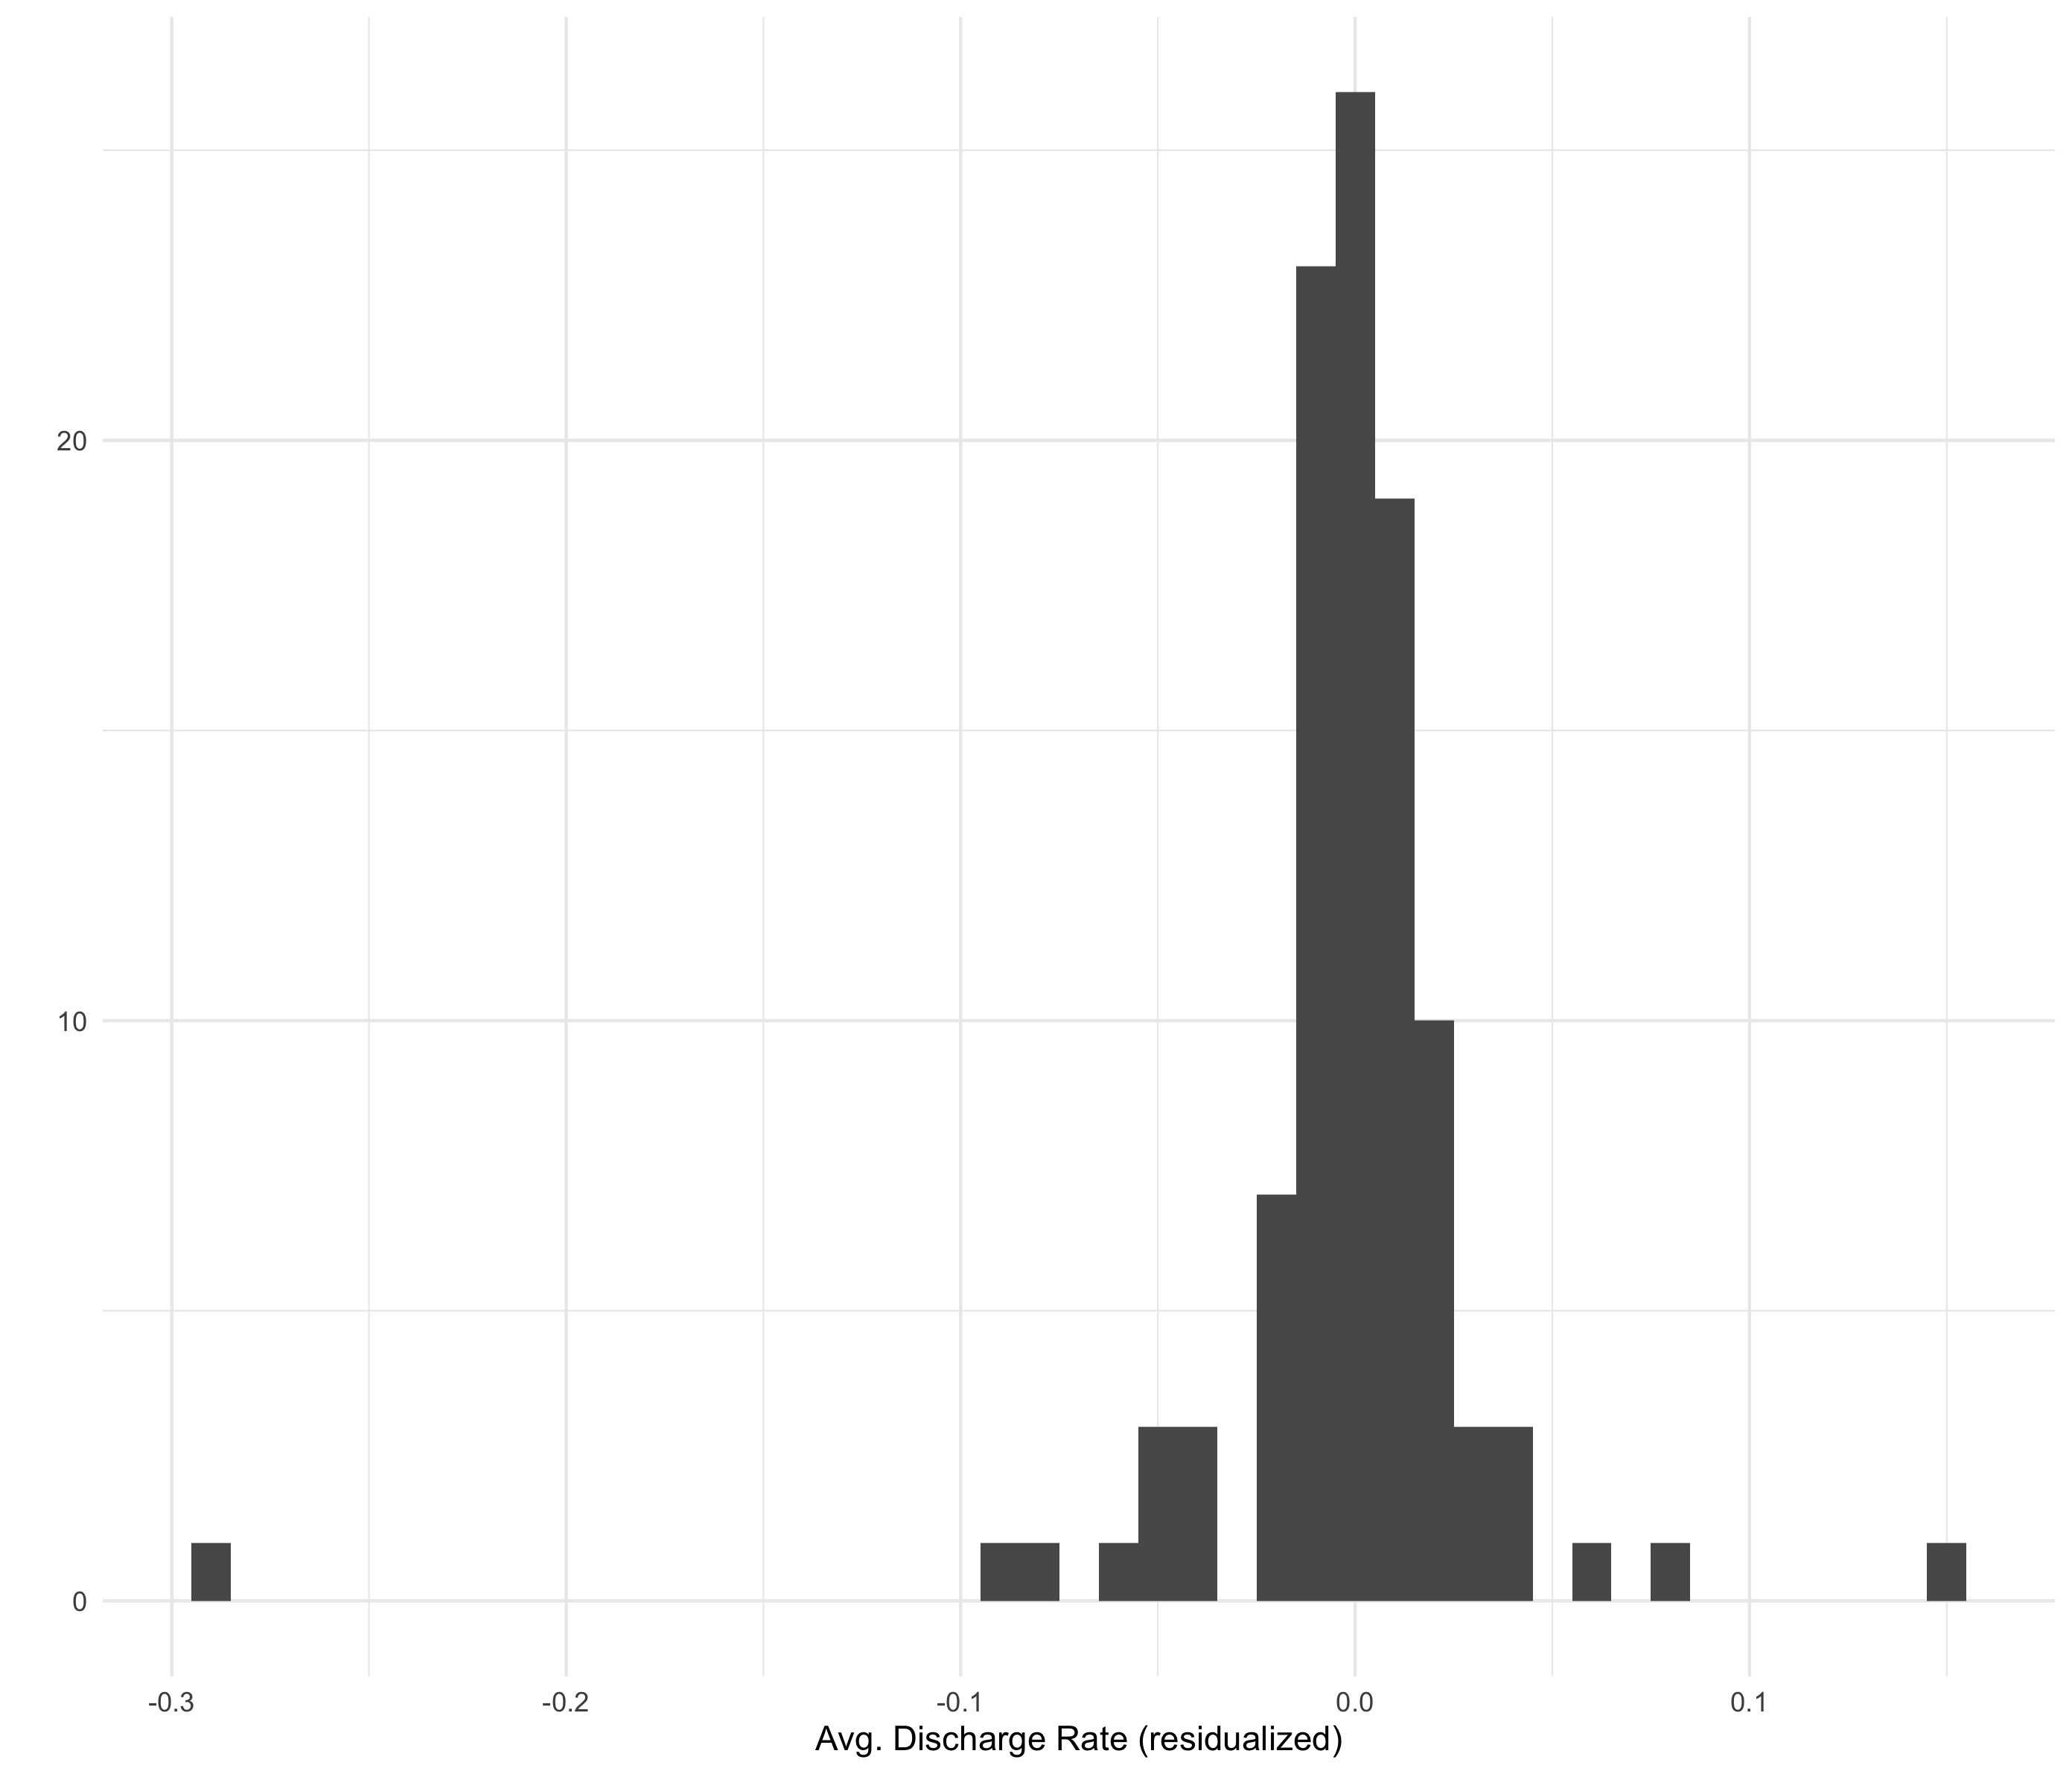
\includegraphics[width=\linewidth]{images/leniency_res.png}
      \end{column}%
    \end{columns}
  \end{frame}

  \begin{frame}{ Important note: Leave-out}
    \begin{itemize}
    \item In practice, individuals use the ``leave-one-out'' mean,
      rather than the actual average
    \item Why? Because if you include your own observation, that will
      be endogeneously correlated
    \item The ``leave-one-out'' leniency is the mechanical solution
      that deals with the many instrument problem
    \end{itemize}
  \end{frame}

  \begin{frame}{ Recall Many IV bias is pernicious}
    \only<1>{    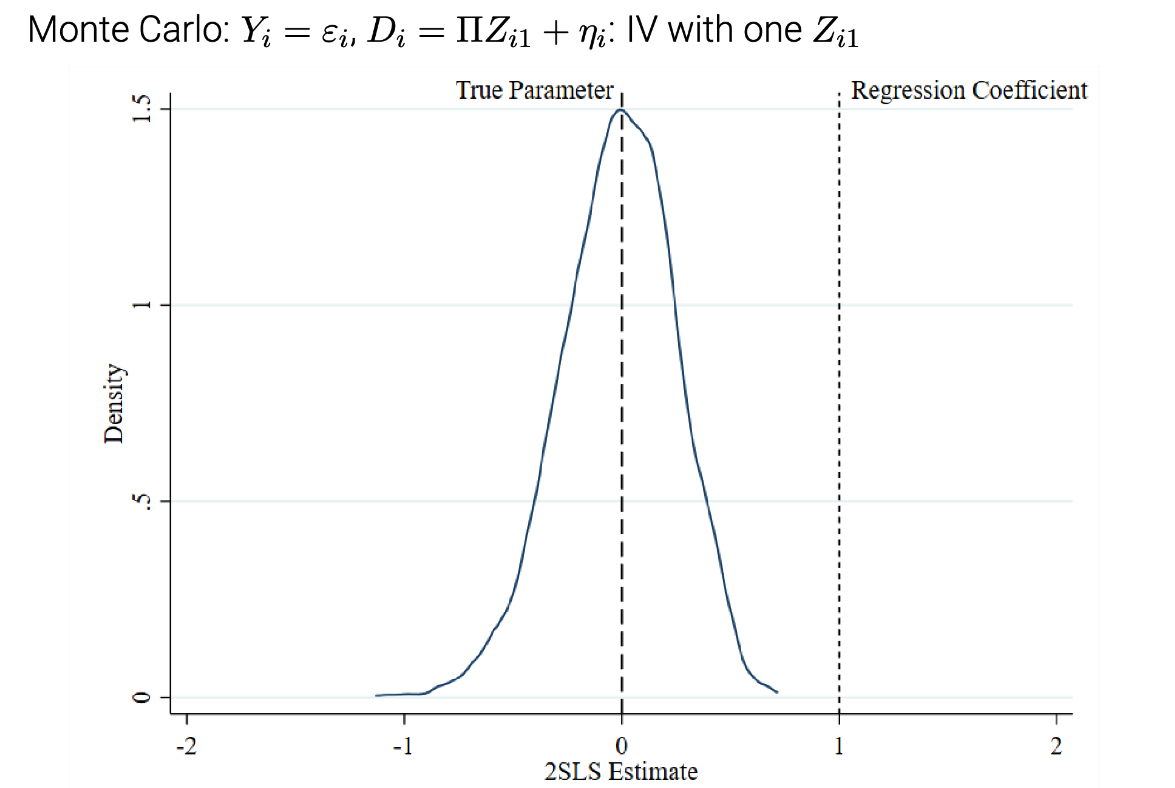
\includegraphics[width=0.7\linewidth]{images/manyiv_hull1.png}    }
    \only<2>{    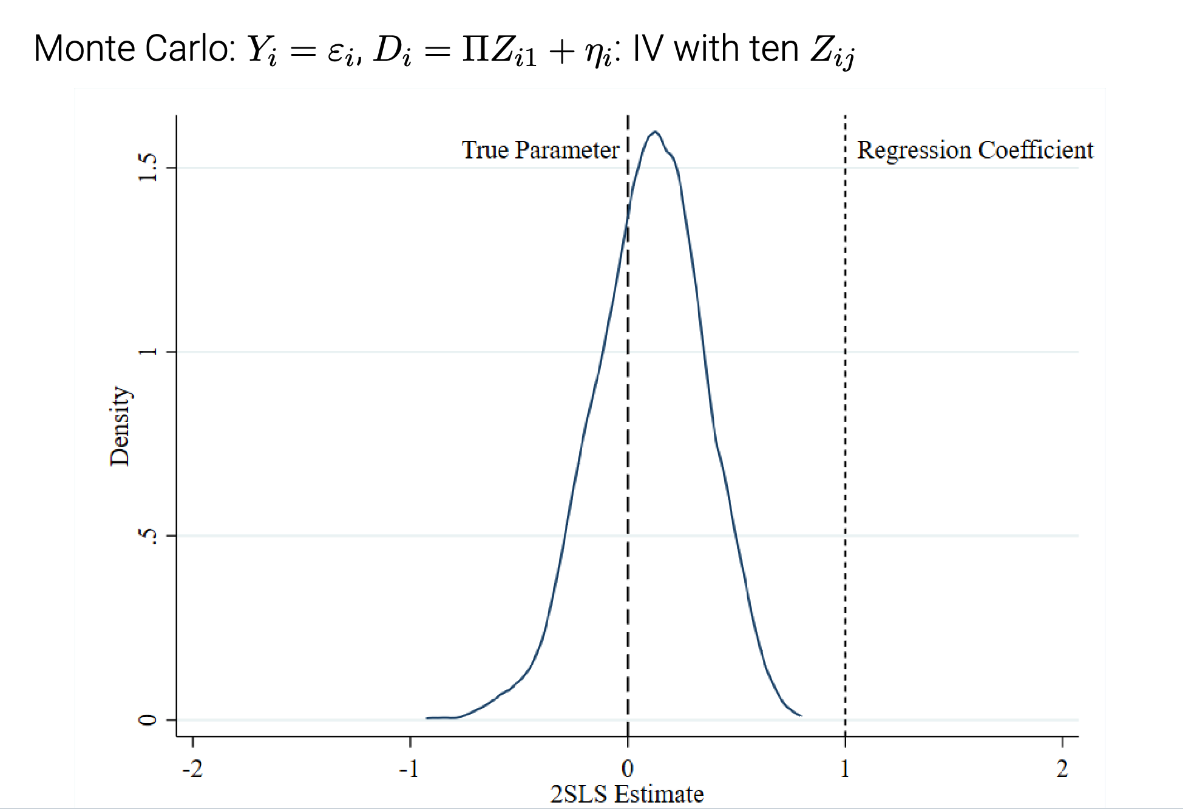
\includegraphics[width=0.7\linewidth]{images/manyiv_hull2.png}    }
    \only<3>{    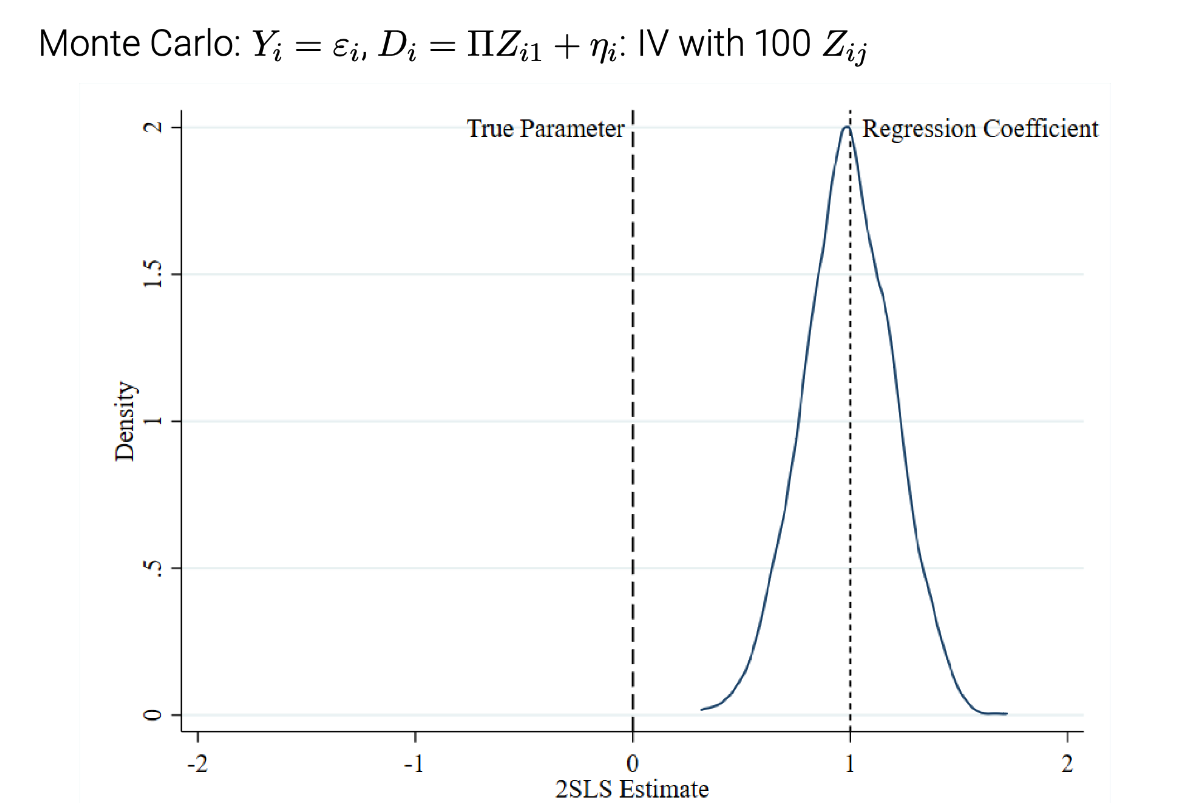
\includegraphics[width=0.7\linewidth]{images/manyiv_hull3.png}    }    
  \end{frame}
  

\begin{frame}{Nothing stops us from doing the same with outcomes!}
    \begin{columns}[onlytextwidth, T] % align columns
      \begin{column}{.5\textwidth}
        \begin{wideitemize}
        \item We can do the same exercise with our outcome measures!
        \item Nothing changes in this setting -- we have both location
          and judge effects, and we can see differences if we don't
          account for them
        \item Location variation absorbs a large chunk, but we still
          see variation in our outcome caused by variation in judges
        \end{wideitemize}
      \end{column}%
      \hfill%
      \begin{column}{.5\textwidth}
        \only<1>{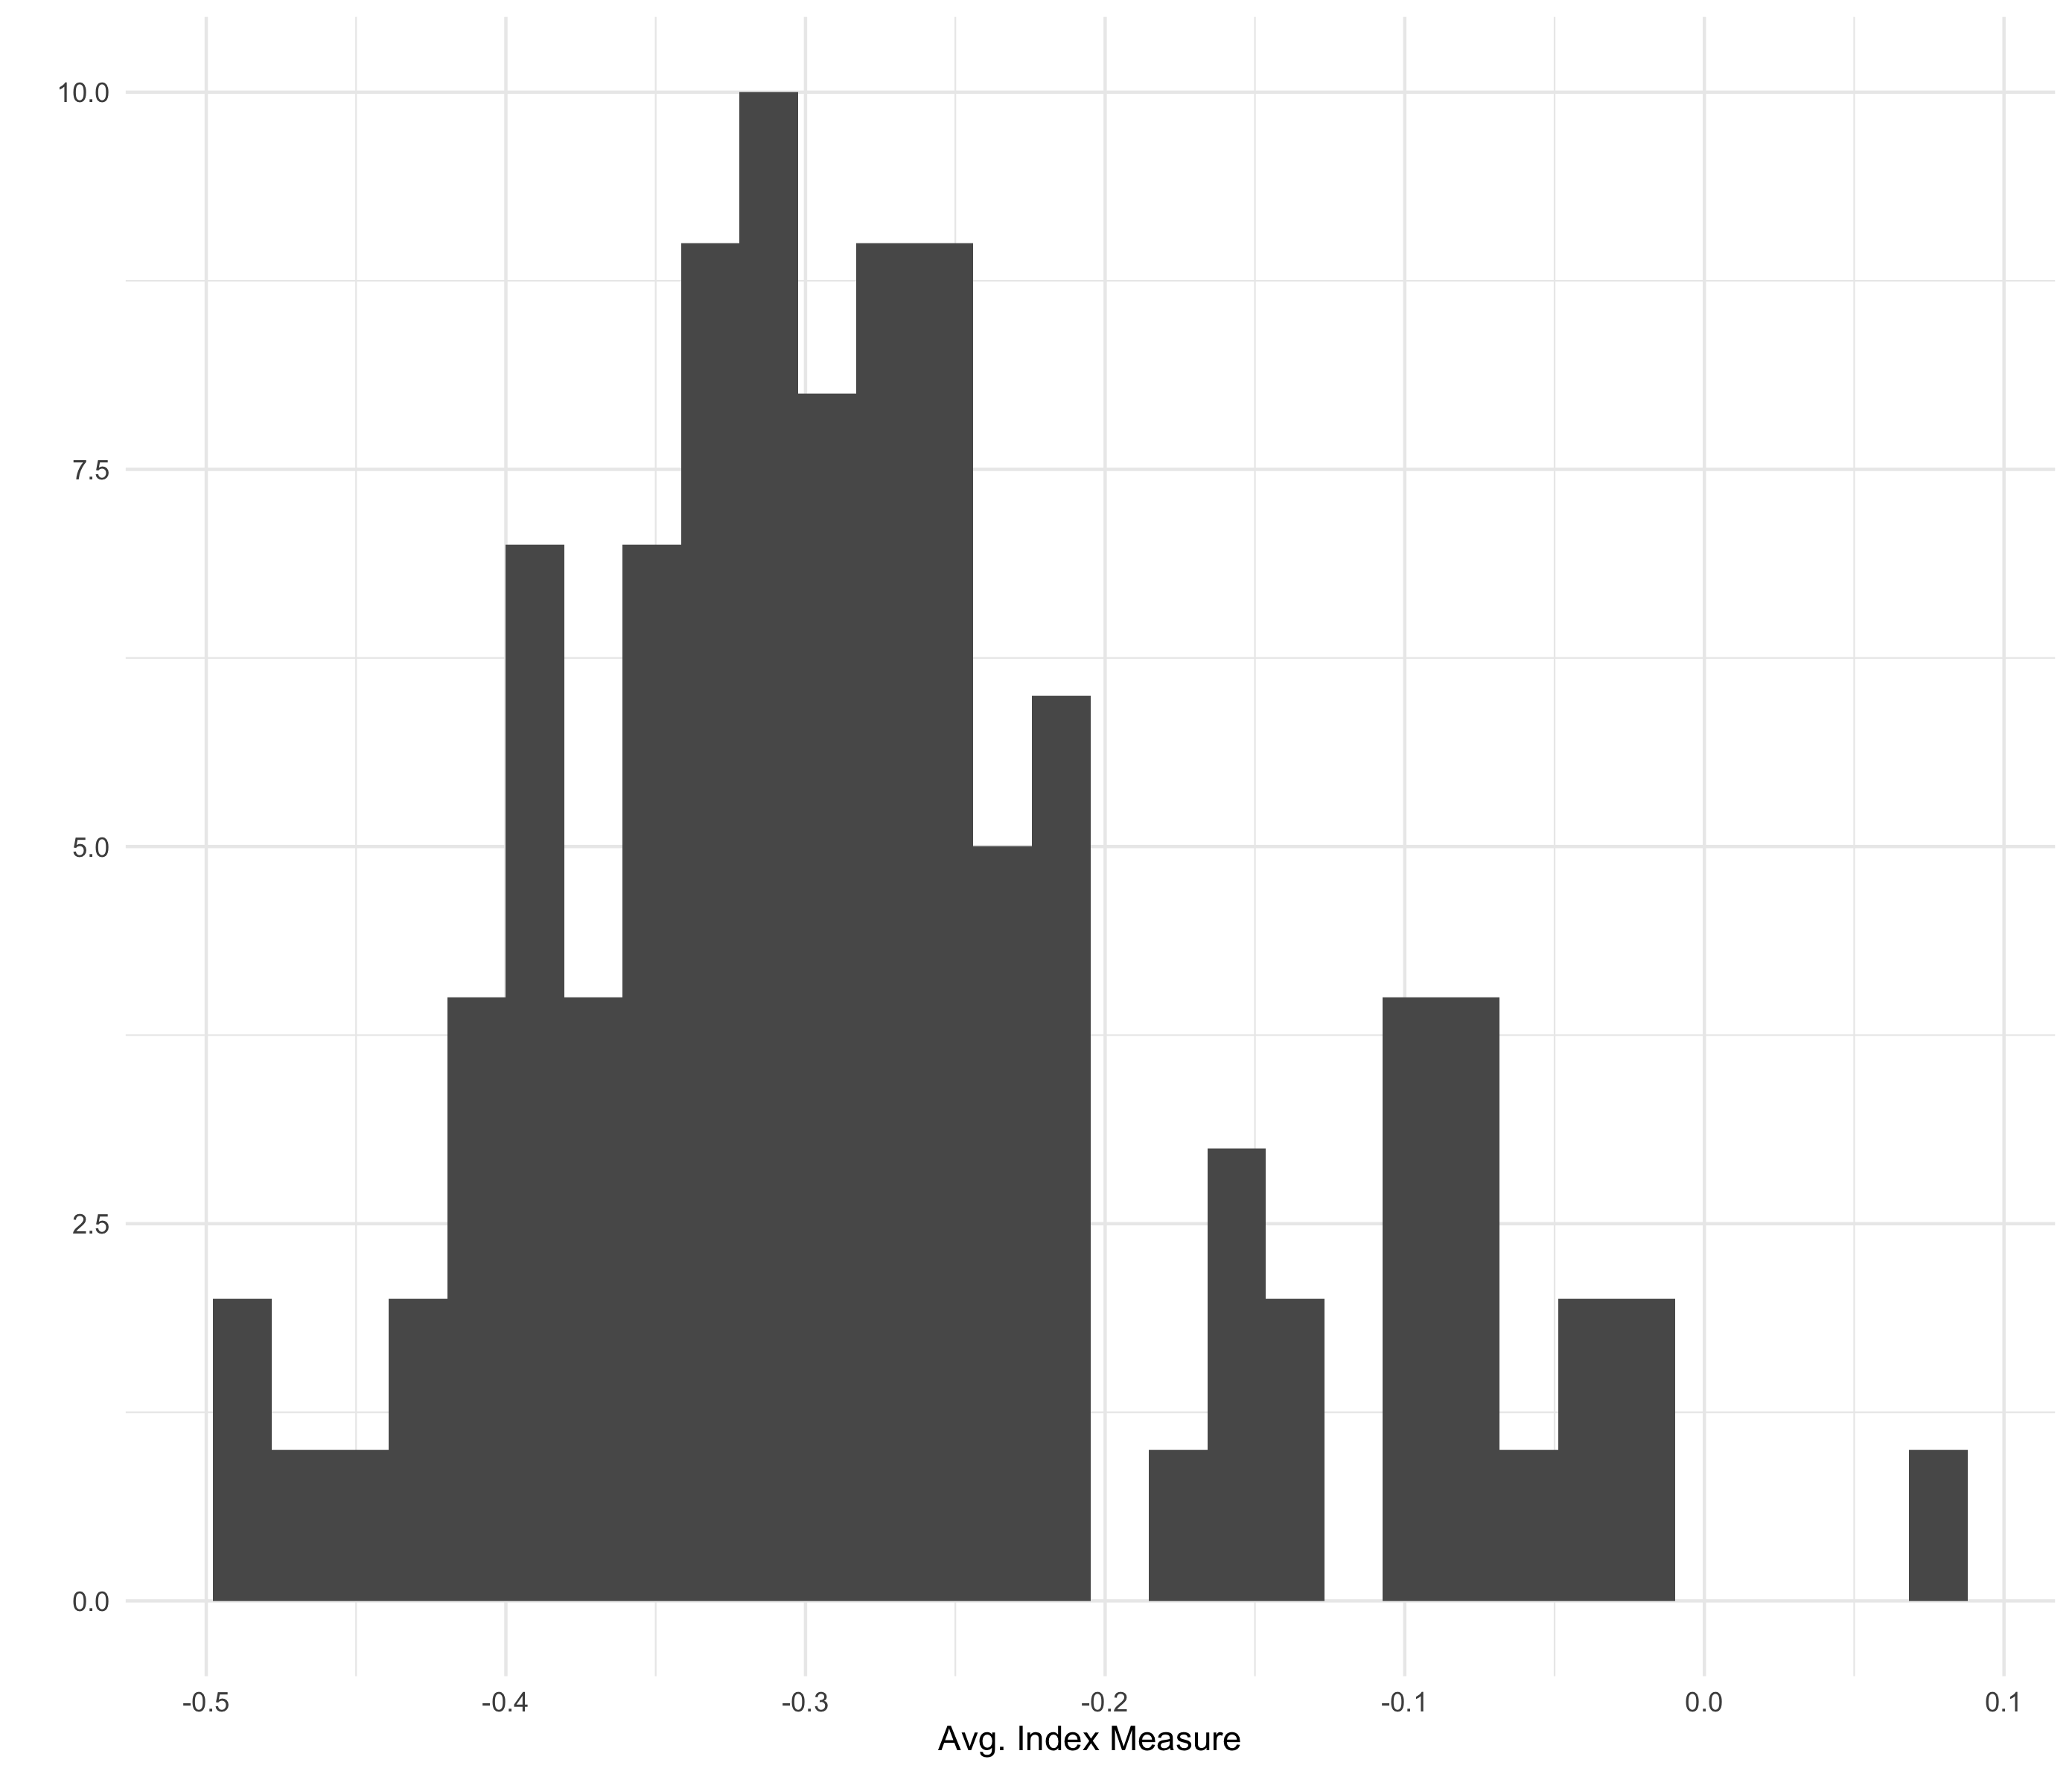
\includegraphics[width=\linewidth]{images/outcome.png}}
        \only<2>{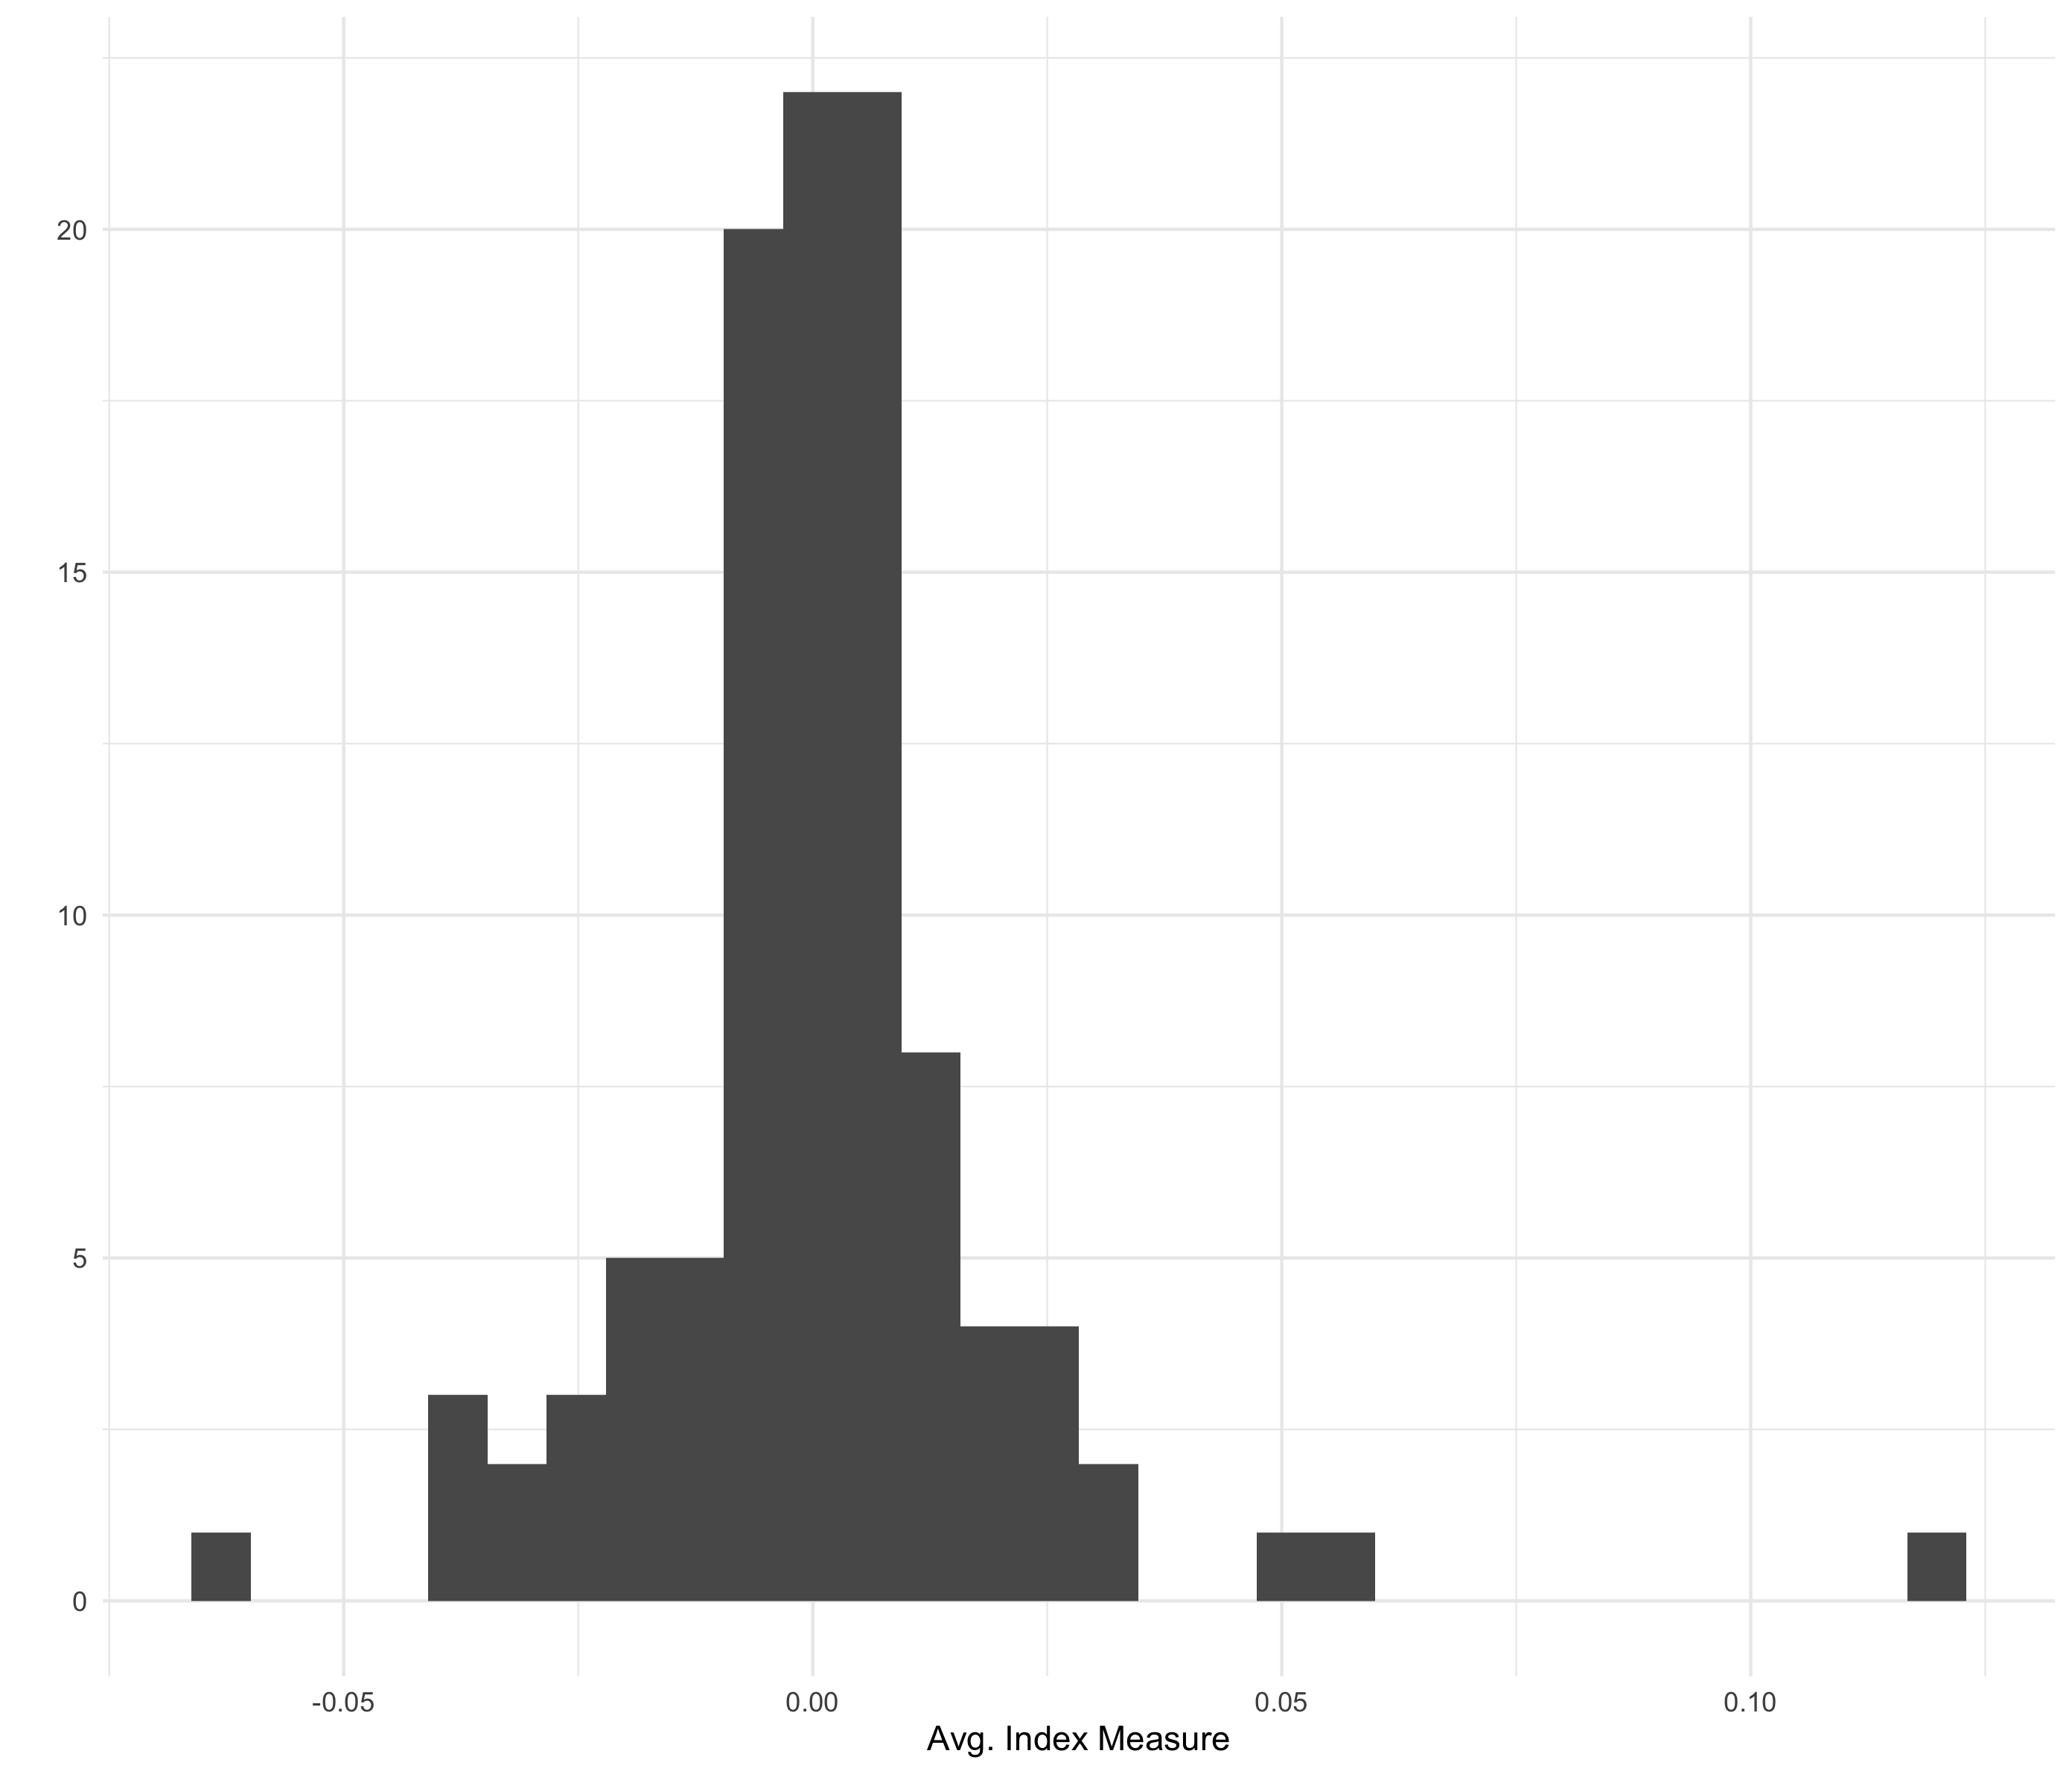
\includegraphics[width=\linewidth]{images/outcome_res.png}}        
      \end{column}%
    \end{columns}
\end{frame}

\begin{frame}{Thinking about instrumental variables}
  \begin{columns}[onlytextwidth, T] % align columns
    \begin{column}{.7\textwidth}
      \begin{wideitemize}
      \item The reason that this is approach is used, of course, is to
        use the variation in $\mu_{D}(q)$ to identify the effect of
        $D$ on $Y$
      \item   So what do we need? Recall
        \begin{enumerate}
          \item  relevance -- e.g. we need that our instrument is predictive of D
          \item exclusion -- e.g. we need that the examiner
            \emph{only} has an effect on Y e.g. potential outcomes
            $Y_{i}(D_{i}(Q_{i}), Q_{i}) = Y_{i}(D_{i}(Q_{i}))$
          \item monotonicity -- e.g. we need an ordering in the effects
          \end{enumerate}
        \item The last two are the challenging part, and not
          inherently testable. Let's discuss the issues, but first,
          how is this done in practice?
      \end{wideitemize}
    \end{column}%
    \hfill%
    \begin{column}{.5\textwidth}
    \end{column}%
  \end{columns}
\end{frame}


\begin{frame}{How is this done in practice, usually?}
  \begin{wideitemize}
  \item In many papers (including my own, historically), the
    \emph{leniency} measure $Z_{i}$ has been used, rather than the
    dummies for judges
  \item Why? A number of reasons:
    \begin{itemize}
    \item Faster -- one time calculation vs. over identifed 2sls
    \item Visualization -- plotting the reduced form and first stage against leniency is very intuitive
    \item Worry about first stage power is easier in the just identified case
    \end{itemize}
  \item But note the following equivalency from our GMM/2SLS estimator:
    \begin{equation}
      \hat{\beta}_{2SLS} = \frac{D'\mathcal{Q}(\mathcal{Q}'\mathcal{Q})^{-1}\mathcal{Q}'Y}{D'\underbrace{\mathcal{Q}(\mathcal{Q}'\mathcal{Q})^{-1}\mathcal{Q}'}_{P_{\mathcal{Q}}}D} = \frac{\hat{D}'Y}{\hat{D}'D} 
    \end{equation}
  \item Using many instruments and using the predicted first stage
    as your instrument are the same thing (adding controls just adds residualization)
  \end{wideitemize}
\end{frame}

\begin{frame}{So which is it?}
  \begin{wideitemize}
  \item Our variation is really the random assignment of $K$
    judges. Collapsing to a predicted first stage doesn't change this,
    and if anything masks the experiement
  \item The estimator is exactly the same (or close, once we deal with
    some estimation issues)
    \begin{itemize}
    \item If this were the right approach, we could do this in every overidentified setting! 
    \end{itemize}
  \item The issue is with inference -- e.g. how much uncertainty is there in the underlying projections?
    \begin{itemize}
    \item Consider the real line with the $\mu_{D}(q)$ and
      $\hat{\mu}_{D}(q)$. Focusing on the estimated leniency measure
      ignores potential important underlying variation in the first stage estimates
    \end{itemize}
  \item In some cases, using the overidentified approach and the
    leniency just-identified approach give very similar standard
    errors -- this is due to relative precision in estimates
    in the $\mu$, and is not guaranteed!
  \end{wideitemize}
\end{frame}

\begin{frame}{An important reason to like leniency measures}
  \begin{wideitemize}
  \item The biggest reason why researchers used the leniency measure
    is it gave a natural way to deal with the ``own-observation''
    problem
  \item Note that $\hat{\mu}_{D}(q)$ includes indivudal $i$'s
    observation in the estimation procedure, scaled by $n^{-1}$
    \begin{itemize}
    \item This term is endogeneous!
    \end{itemize}
  \item Leniency measures that researchers construct use a
    ``leave-one-out'' mean to account for this, and instead measure an
    individual's leniency exposure as a judge's leniency
    \emph{excluding} own observation
  \item This variable was easily plugged into 2SLS and avoided the bias
  \item But... this approach just approximates jackknife IV!
    \begin{itemize}
    \item This own observation issue is exactly the bias that came up from overidentified IV in finite samples
    \item When the number of judges is large-ish within a court, this
      can be an issue
    \end{itemize}
  \end{wideitemize}
\end{frame}


\begin{frame}{Use (U)JIVE!}
  \begin{wideitemize}
  \item Given the leniency approach is exactly solved with a known technique, there is
    no great reason to use leniency directly
  \item It is more transparent to use the judge variation directly
  \item If you want to do graphical visualization, just use the first stage coefficients!
  \item A key issue raised in Kolesar (2013) is the issue of many controls (e.g. many fixed effects) which creates the same problem as many instruments under certain settings
    \begin{itemize}
    \item Provides a solution, through UJIVE. See his website for
      code.
    \end{itemize}
  \end{wideitemize}
\end{frame}


\begin{frame}{How to test these exclusion and monotonoicity?}
  \begin{columns}[onlytextwidth, T] % align columns
    \begin{column}{.5\textwidth}
      \begin{wideitemize}
      \item Testing exclusion is always challenging
      \item However, like standard treatment designs and RCTs, we can test for balance
      \item Use the predicted first stage (e.g. the propensity score)
        and test of excluded covariates across p-scores $\hat{\mu}_{D}(q)$
      \item See Aronow and Miller for discusion on balance tests
      \end{wideitemize}
    \end{column}%
    \hfill%
    \begin{column}{.5\textwidth}
      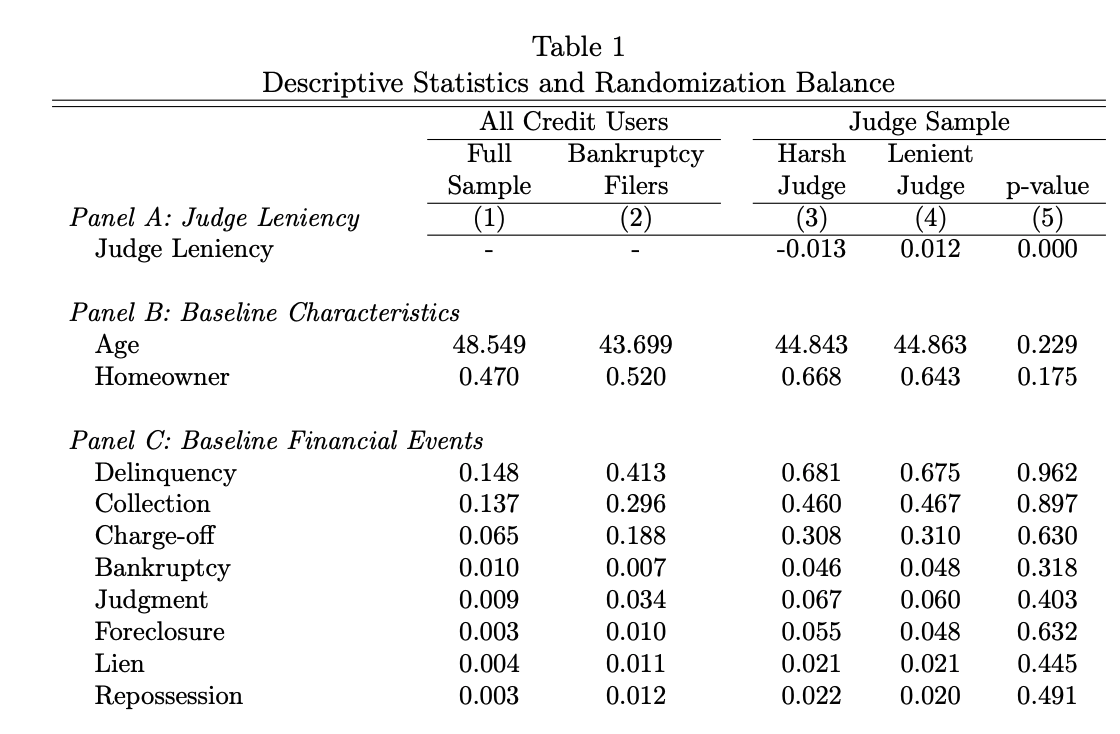
\includegraphics[width=\linewidth]{images/dgy_3.png}
    \end{column}%
  \end{columns}
  
\end{frame}

\begin{frame}{How to test these exclusion and monotonoicity?}
  \begin{columns}[onlytextwidth, T] % align columns
    \begin{column}{.5\textwidth}
      \begin{wideitemize}
      \item<1-> Testing (and believing) monotonicity is also challenging
      \item<2-> Kitagawa (2015) and Frandsen et al. (2019) discuss ways to
        test this for binary outcomes
      \item<2-> Current limitation is finite sample approximation
      \item<2-> However, provide useful intuititon for tests
      \end{wideitemize}
    \end{column}%
    \hfill%
    \begin{column}{.5\textwidth}
      \only<1>{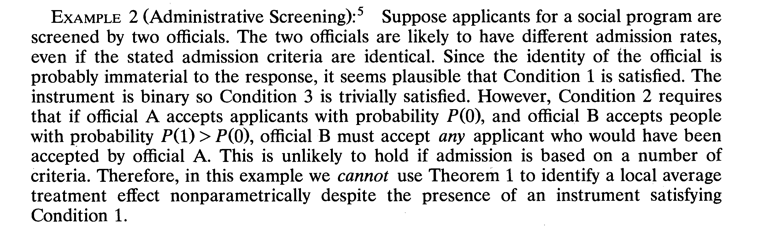
\includegraphics[width=\linewidth]{images/imbensangrist_judge.png}}
\only<2>{      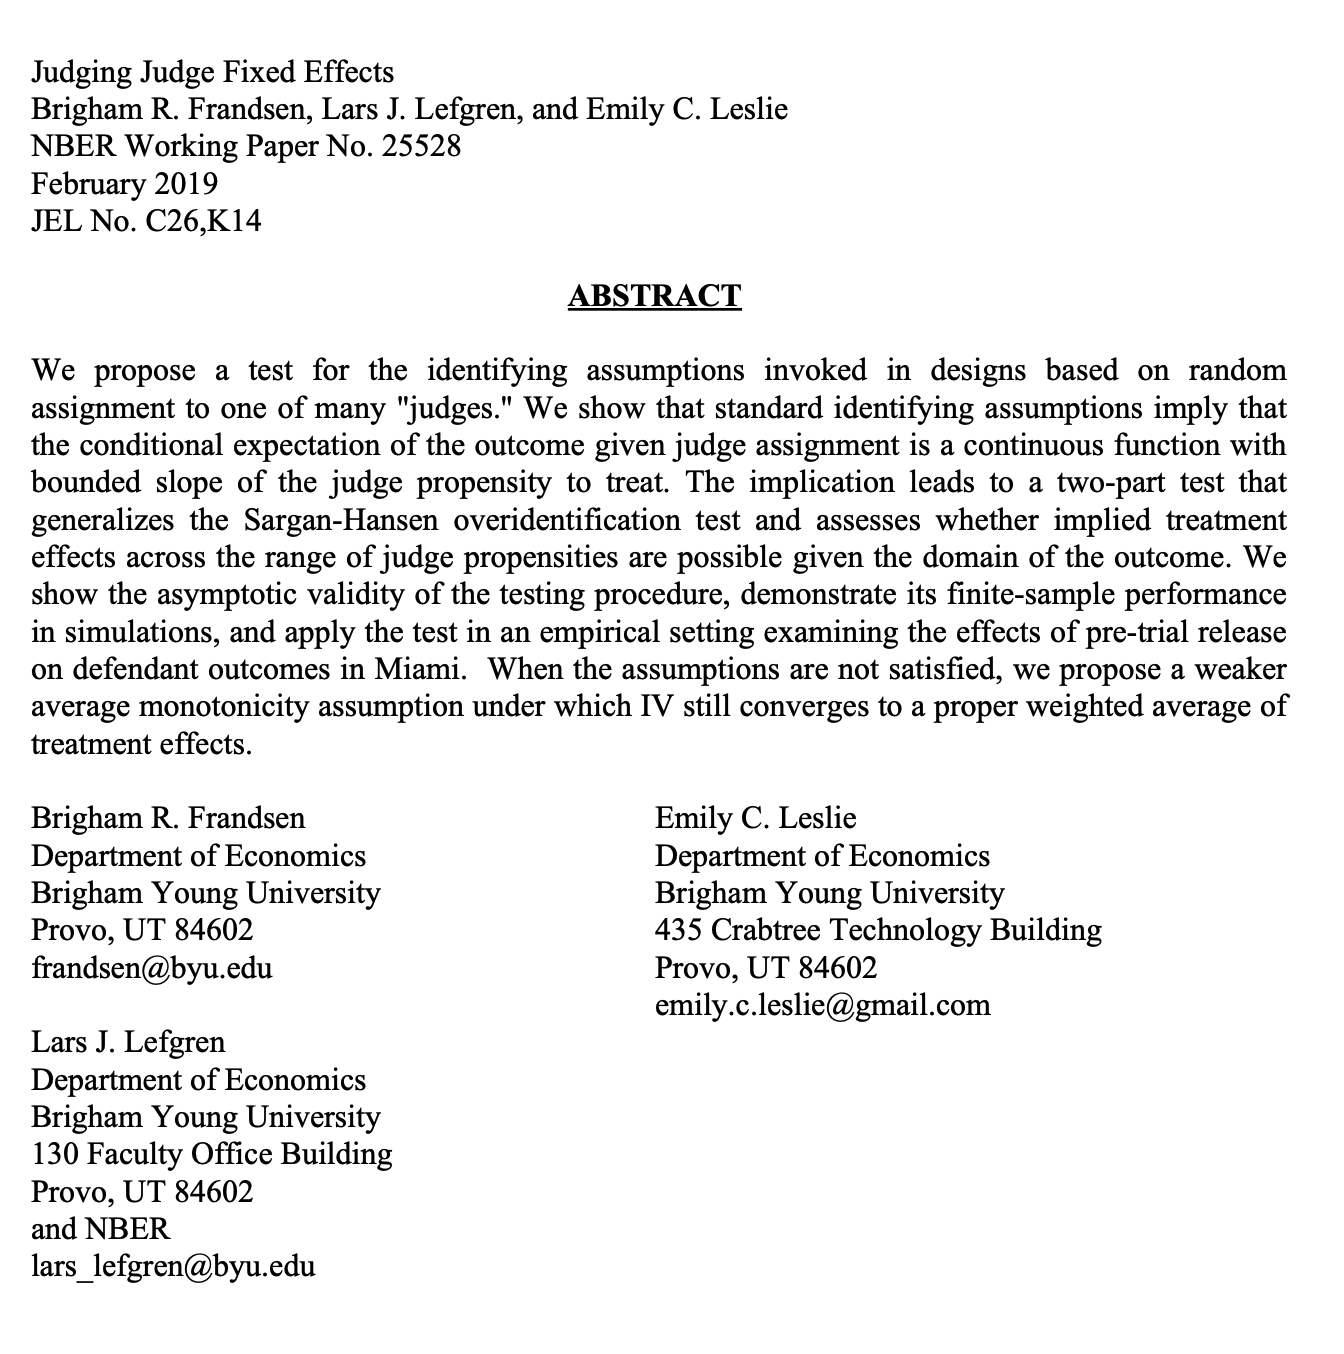
\includegraphics[width=\linewidth]{images/jjfe_1.png}}
    \end{column}%
  \end{columns}
\end{frame}


\begin{frame}{Kitagawa (2015) result}
  \begin{columns}[onlytextwidth, T] % align columns
    \begin{column}{.5\textwidth}
      \begin{itemize}
      \item Consider binary endogeneous treatment $D$ and a discrete instrument $Z$.
      \item Joint \emph{testable} assumption: instrument is valid and monotonicity. Why?
        \begin{itemize}
        \item Consider $p(y,d) = Pr(Y = y, D = d | Z = 1)$, $q(y,d) = Pr(Y = y, D = d | Z = 0)$
        \item Let $P$ and $B$ be the probability over sets
        \item Imbens and Rubin (1997) show
          \vspace{-10pt}
          \begin{align*}
            P(B, 1) - Q(B,1) &= Pr(Y_{1} \in B, D_{1} > D_{0})\\
            P(B, 0) - Q(B,0) &= Pr(Y_{0} \in B, D_{1} > D_{0})\\                        
          \end{align*}
        \end{itemize}
        \vspace{-10pt}                
      \item Testable implication:
          \vspace{-10pt}        
          \begin{align*}
            P(B, 1) - Q(B,1) &\geq 0\\
            P(B, 0) - Q(B,0) &\geq 0
          \end{align*}
      \end{itemize}
    \end{column}%
    \hfill%
    \begin{column}{.5\textwidth}
            \only<1>{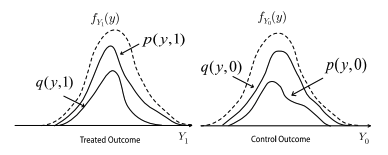
\includegraphics[width=\linewidth]{images/kitagawa_valid.png}}
            \only<2>{      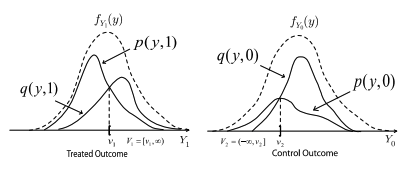
\includegraphics[width=\linewidth]{images/kitagawa_invalid.png}}
    \end{column}%
  \end{columns}
\end{frame}

\begin{frame}{Extension to Examiner designs (Frandsen et al.)}
  \begin{columns}[onlytextwidth, T] % align columns
    \begin{column}{.5\textwidth}
      \begin{itemize}
      \item Now, with multiple judges, we don't know the ``true'' $z$ values
      \item Need to instead consider how this moves with noise
      \item Mapping from judges to ``leniency'' and then use Kitagawa test
        \item Package available: \texttt{testjfe} in Stata
      \end{itemize}
    \end{column}%
    \hfill%
    \begin{column}{.5\textwidth}
    \end{column}%
  \end{columns}
\end{frame}


\begin{frame}{Brief aside on inference}
  \begin{wideitemize}
  \item The many instruments field is still working on heteroskedasticty and complicated inference settings
  \item This stuff is challenging!
  \item However, given that the random assignment is effectively a set
    of judges to a given individual, robust standard errors seems most appropriate
  \item However, the norm (requested by referees, etc.) appears to be judge clustering 
    \begin{itemize}
    \item   Not totally clear why
    \end{itemize}
  \end{wideitemize}
\end{frame}

\begin{frame}{Further Readings}
  \begin{wideitemize}
  \item Cunningham (2021) chapter 7.8.2
  \item Judging Judge Fixed Effects (2020)
  \item Mueller-Smith (2015)
  \item Dobbie and Song (2015)
  \end{wideitemize}
\end{frame}

\end{document}